% build with: pdflatex --shell-escape fig.tex
\documentclass[tikz, convert={density=800}]{standalone}

\usepackage{tikz}
\definecolor{myOrange}{HTML}{ffa500}
\definecolor{myBlue}{HTML}{42affa}

\begin{document}
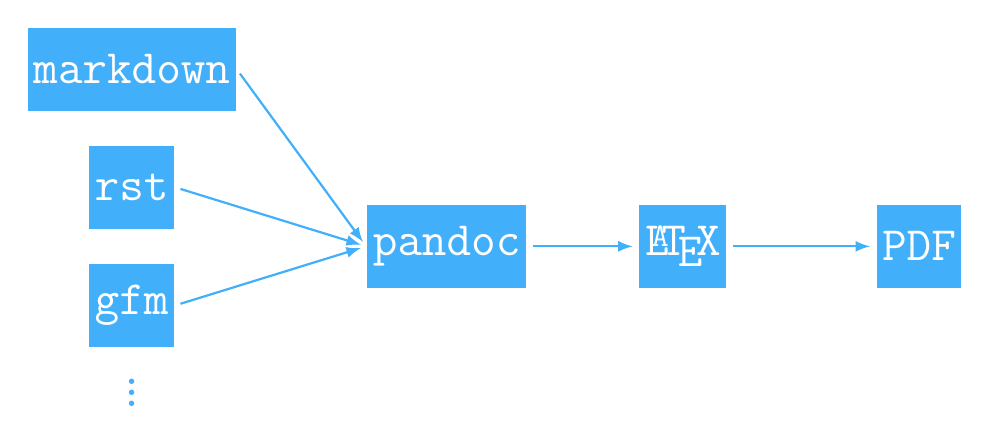
\begin{tikzpicture}[>=latex, thick, shorten >=2pt, shorten <=2pt, ->, myBlue]

%  \tikzstyle{C}=[circle,fill=myBlue,text=white,minimum size=30pt,inner sep=2pt, font=\LARGE]
  \tikzstyle{C}=[rectangle,fill=myBlue,text=white,minimum size=30pt,inner sep=2pt, font=\LARGE]
  \tikzstyle{M}=[circle,fill=myOrange,text=white,minimum size=30pt,inner sep=2pt, font=\LARGE]
  \tikzstyle{B}=[text=myBlue, font=\LARGE]

  \node[C] at (-2,3) (markdown) {\texttt{markdown}};
  \node[C] at (-2,1.5) (rst) {\texttt{rst}};
  \node[C] at (-2,-0.0) (gfm) {\texttt{gfm}};
  \node[B] at (-2,-1.) (dots) {\texttt{\vdots}};

  
  \node[C] at (2,0.75) (pandoc) {\texttt{pandoc}};
  \node[C] at (5,0.75) (latex) {\texttt{\LaTeX}};
  
  \node[C] at (8,0.75) (pdf) {\texttt{PDF}};
  
  \draw [] (markdown.east) to (pandoc.west);
  \draw [] (rst.east) to (pandoc.west);
  \draw [] (gfm.east) to (pandoc.west);
  
  \draw [] (pandoc.east) to (latex.west);
  \draw [] (latex.east) to (pdf.west);
  
%  \draw [] (pandoc.east) to (markdownR.west);
%  \draw [] (pandoc.east) to (rstR.west);
%  \draw [] (pandoc.east) to (gfmR.west);
%  \draw [] (pandoc.east) to (manR.west);
%  \draw [] (pandoc.east) to (docxR.west);
  
  
\end{tikzpicture}
\end{document}
